%%%%%%%%%%%%%%%%%%%%%%%%%%%%%%%%%%%%%%%%%%

\chapter{Tests of the second switcher and switcher wye on the West Beamline}\label{chap:fall2021}

%%%%%%%%%%%%%%%%%%%%%%%%%%%%%%%%%%%%%%%%%%

In 2021, the ongoing construction of the \acrshort{msr} (Sec.~\ref{sec:MSR}) relegated the commissioning of nEDM components to the West beamline (Fig.~\ref{fig:AreaB_schematic}). A second rotary switcher and a new ``switcher wye'' guide segment for connecting both switchers to the beamline (Fig.~\ref{subfig:switcher_mockup}) were tested. We performed measurements to determine the quality of the \ucn and \ucn spin transport in these components.

%%%%%%%%%%%%%%%%%%%%%%%%%%%%%%%%%%%%%%%%%%%%%%

\section{Description of experimental setup (2021)}\label{sec:2021_experimental_setup}

%%%%%%%%%%%%%%%%%%%%%%%%%%%%%%%%%%%%%%%%%%%%%%

\begin{figure}[h]
    \centering
    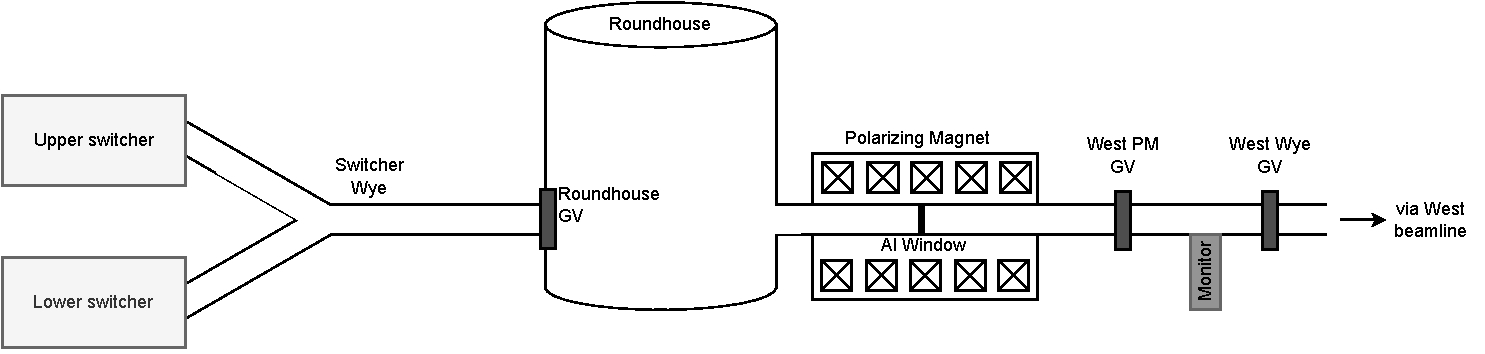
\includegraphics[width=\textwidth]{figures/westbeamline_2021.pdf}
    \caption[West beamline configuration for measurements in 2021.]
    {West beamline configuration for measurements in 2021. A single channel spin analyzer was located on the lower switcher, and simultaneous spin analyzer was located on the upper switcher. Beam height detectors were rearranged for different measurements as per Sec.~\ref{sec:2021_ucn_transport_switchers}.}\label{fig:west_beamline_2021}
\end{figure}

The West beamline hosts the UCN$\tau$ neutron lifetime experiment, which unlike the North beamline contains a buffer volume referred to as the ``roundhouse.'' The roundhouse was introduced in 2018 to smooth temporal fluctations in the UCN production rate during the UCN$\tau$ filling period~\cite{gonzalez_ucn_tau}. When the UCN$\tau$ experiment is collecting production data, the roundhouse contains a neutron absorber located \qty{1}{m} above beam height to precondition the input \ucn energy spectrum. The absorber was removed for the measurement cycle. 

The switcher wye consists of NiP-coated Al guide that branches from a stem (\qty{4}{in} inner-diameter (ID)) into two arms (\qty{3}{in} ID). Arms of the wye were connected to two rotary switchers (Sec.~\ref{sec:lanl_switchers}) mounted on a switcher stand, with dimensions shown in Fig.~\ref{fig:switcher_stand_measurements}. Vertical separation between the switchers was $\qty{19.6}{in}\approx \qty{0.5}{m}$, which provides a $\approx \qty{25}{neV}$ gravitational potential step for \ucn to reach the elevated switcher.

The newly constructed second switcher was placed on the lower side of the switcher stand. As in Fig.~\ref{subfig:west_beamline_switchers}, the single channel spin analyzer (Chaps.~\ref{chap:north_beamline_paper}--\ref{chap:ssa_2020}) was mounted to the second switcher. The previously characterized rotary switcher was mounted on the elevated platform of the switcher stand. Rotary switchers are hereafter designated as ``upper switcher'' and ``lower switcher'' based on their relative positions on the switcher stand.

\BZnS scintillator (\qty{3}{in} diameter) \ucn detectors, referred to as ``beam height detectors,'' were mounted to ports on either upper or lower switcher as needed.


\begin{figure}
\centering
%subfigure width gets "multiplied" by includegraphics width
\begin{subfigure}{.5\textwidth}
  \centering
  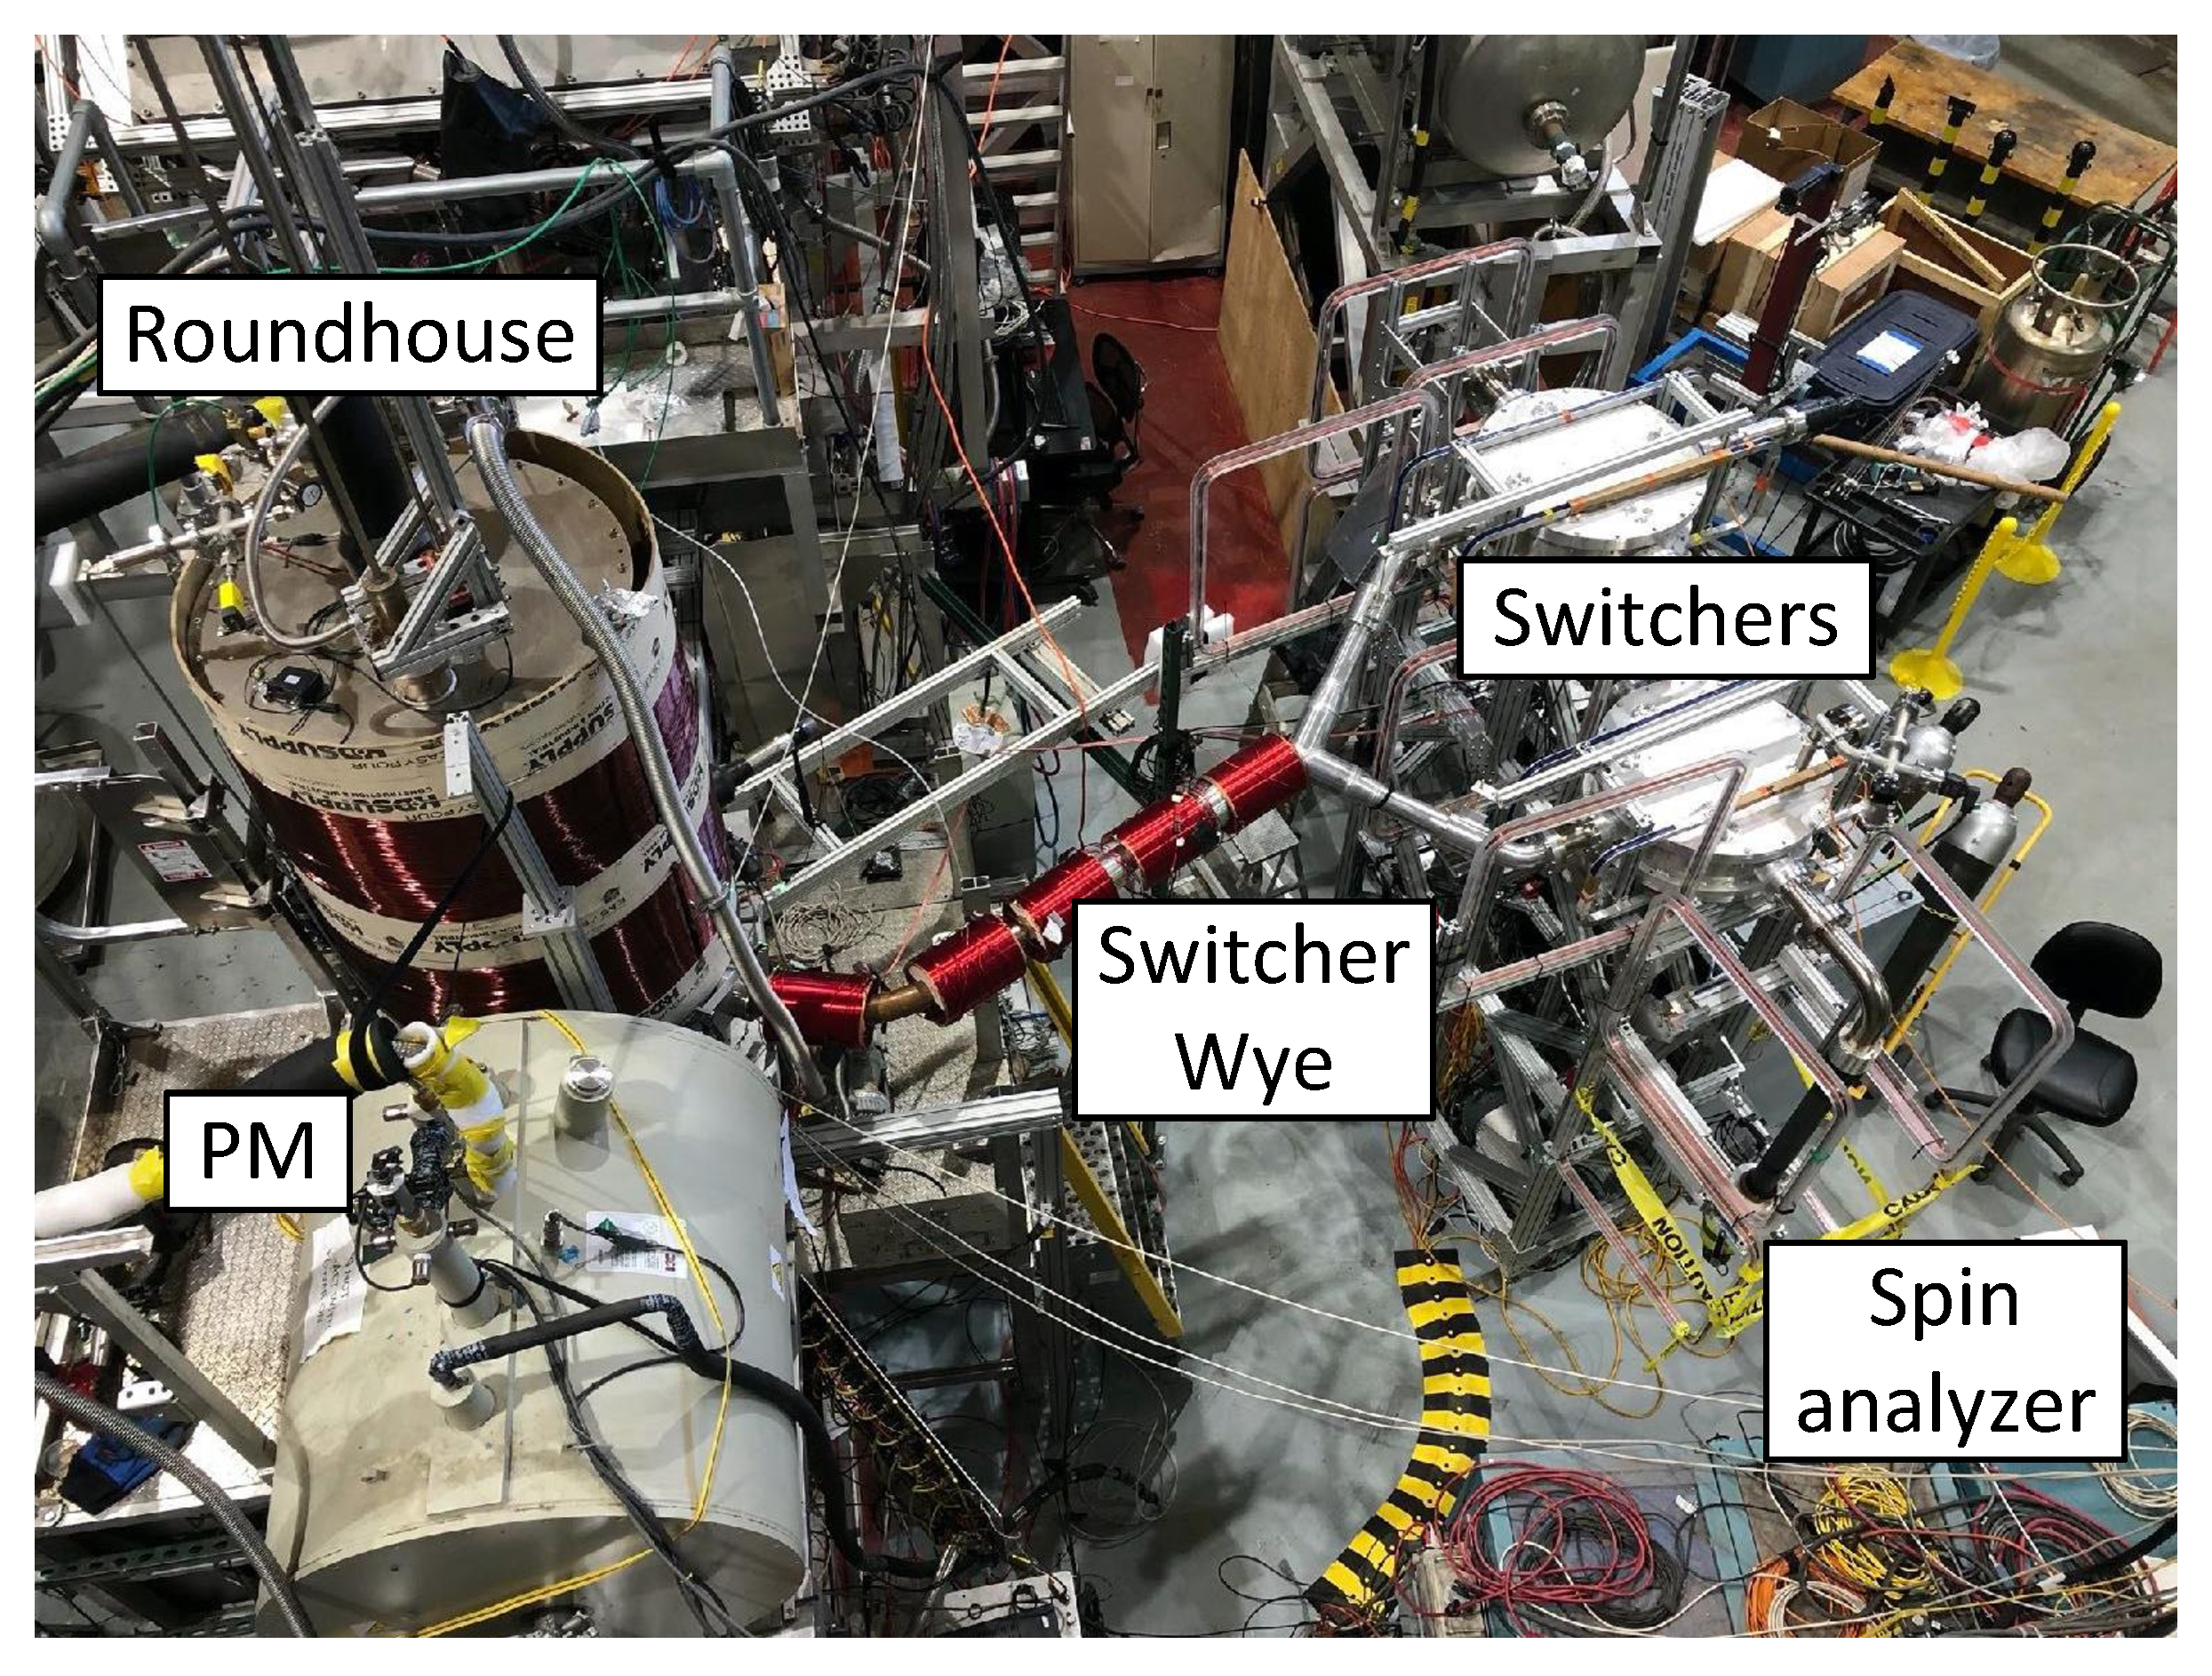
\includegraphics[width=\textwidth]{figures/2021_west_beamline_image.pdf}
  \vspace{5pt}
  \caption{}\label{subfig:west_beamline_switchers}
\end{subfigure}%DO NOT REMOVE THIS '%'
\begin{subfigure}{.5\textwidth}
  \centering
  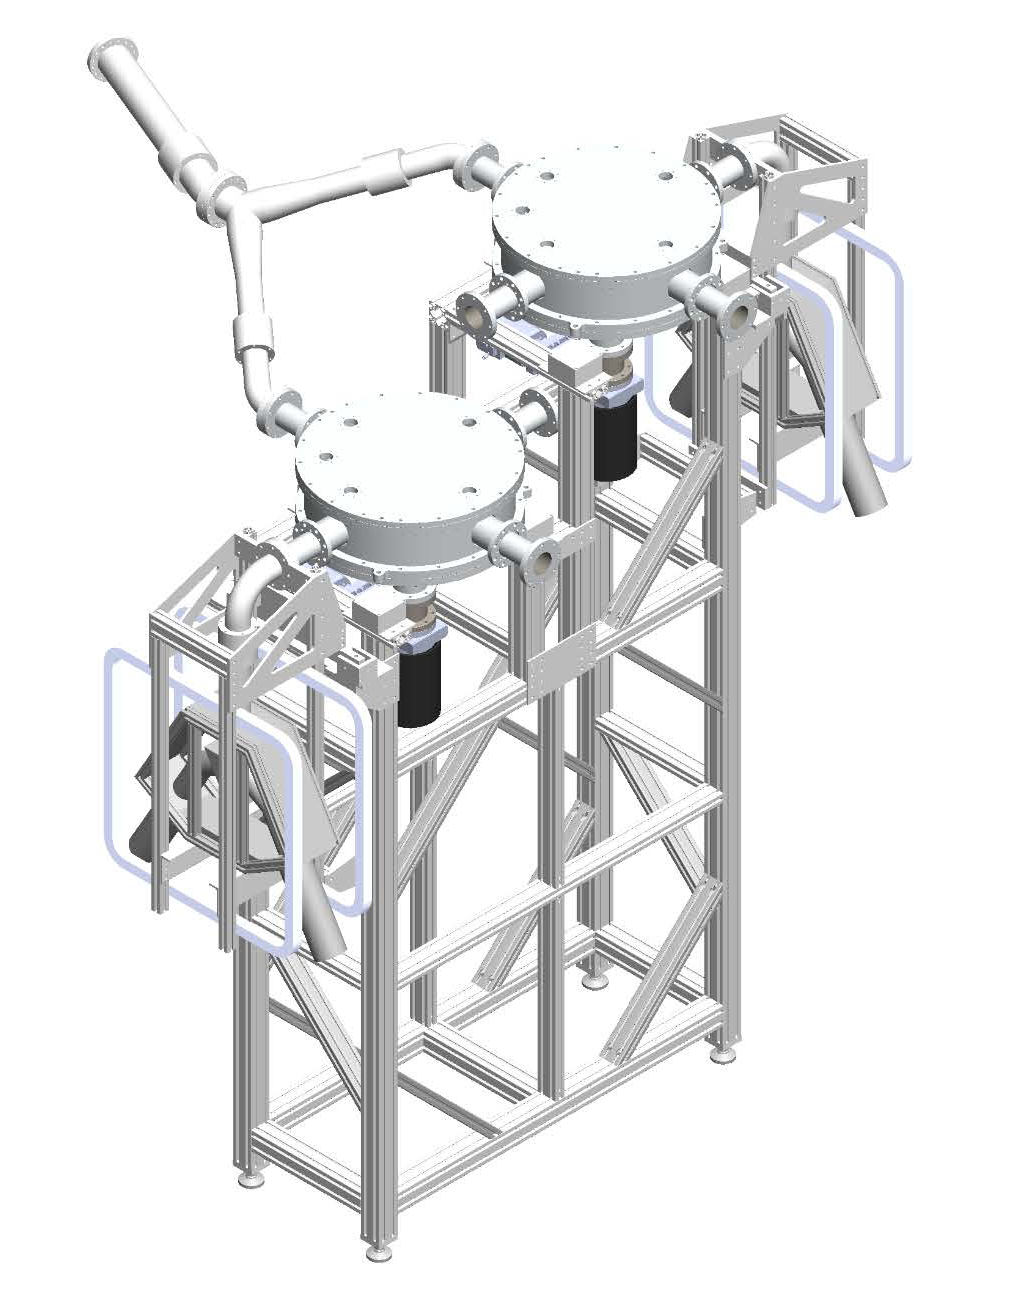
\includegraphics[height=3in]{figures/switcher_mockup.png}
  \caption{}\label{subfig:switcher_mockup}
\end{subfigure}
\caption
{\textbf{(\subref{subfig:west_beamline_switchers})} Image of the experimental setup on the West beamline. \textbf{(\subref{subfig:switcher_mockup})} Rendering of the switcher wye, switcher stand, and switcher, depicted here with simultaneous spin analyzers attached.}
\label{fig:west_beamline_switchers}
\end{figure}

\begin{sidewaysfigure}
    \centering
    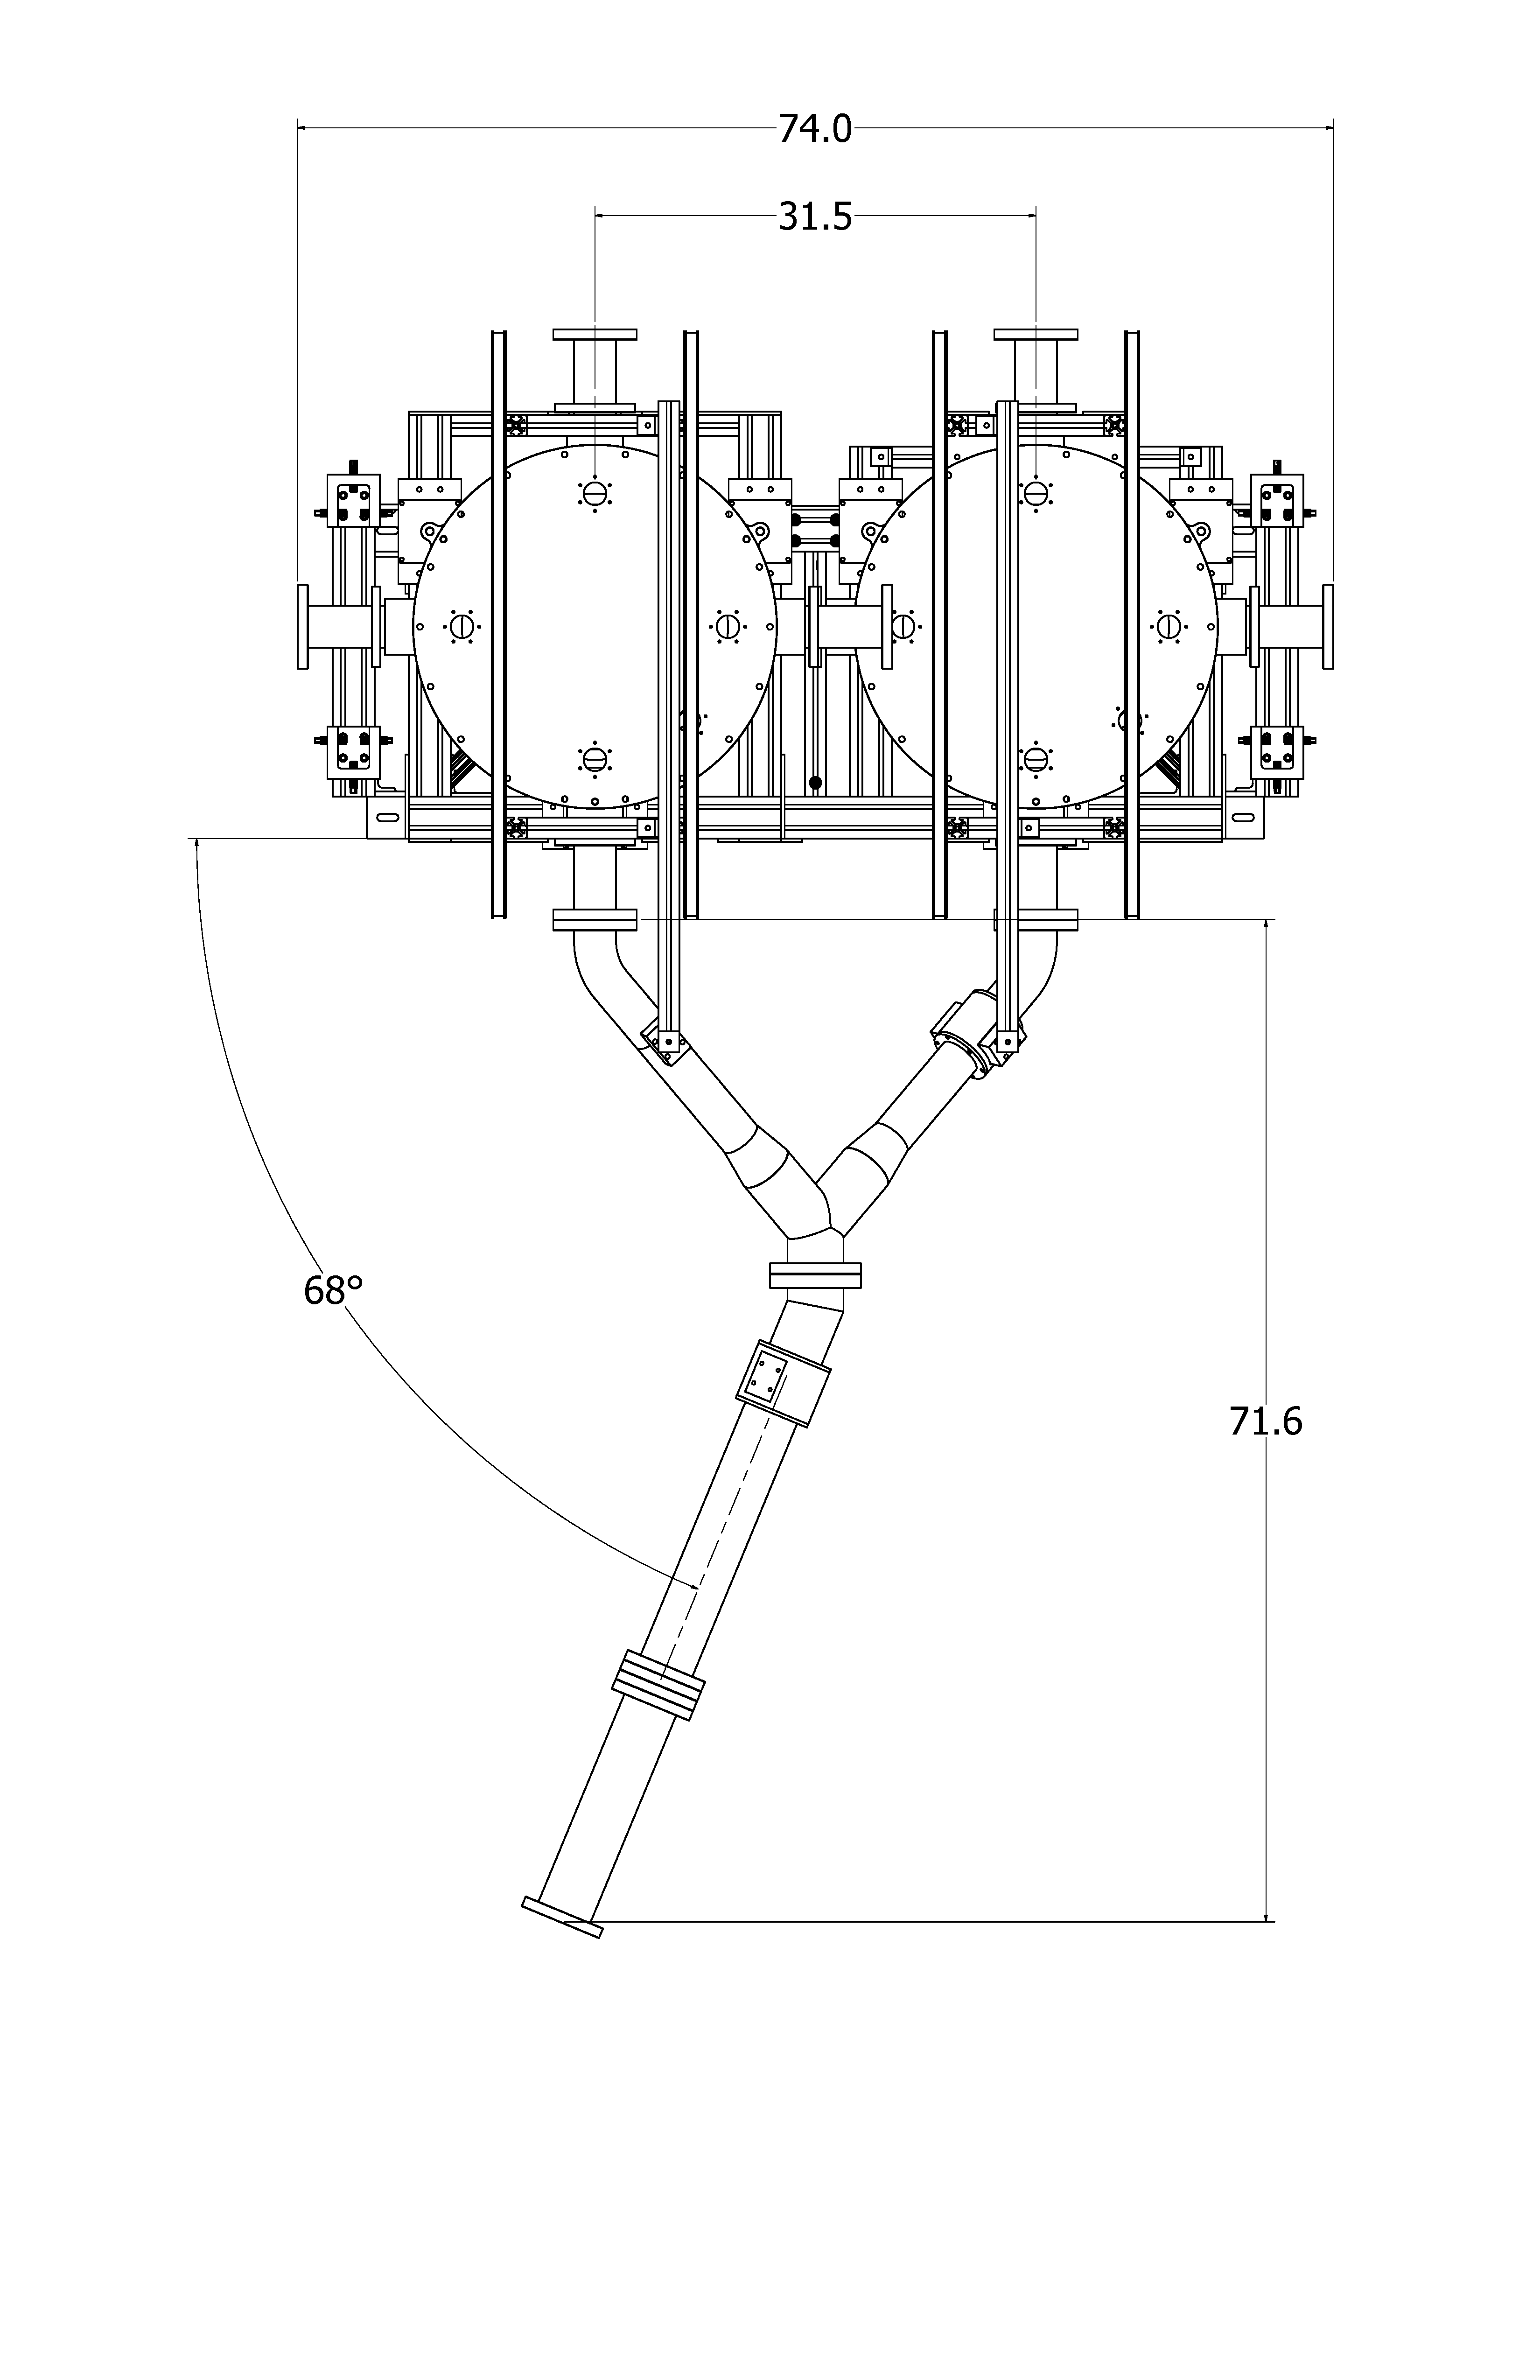
\includegraphics[width=3.5in]{figures/switcher_horizontals.pdf}
    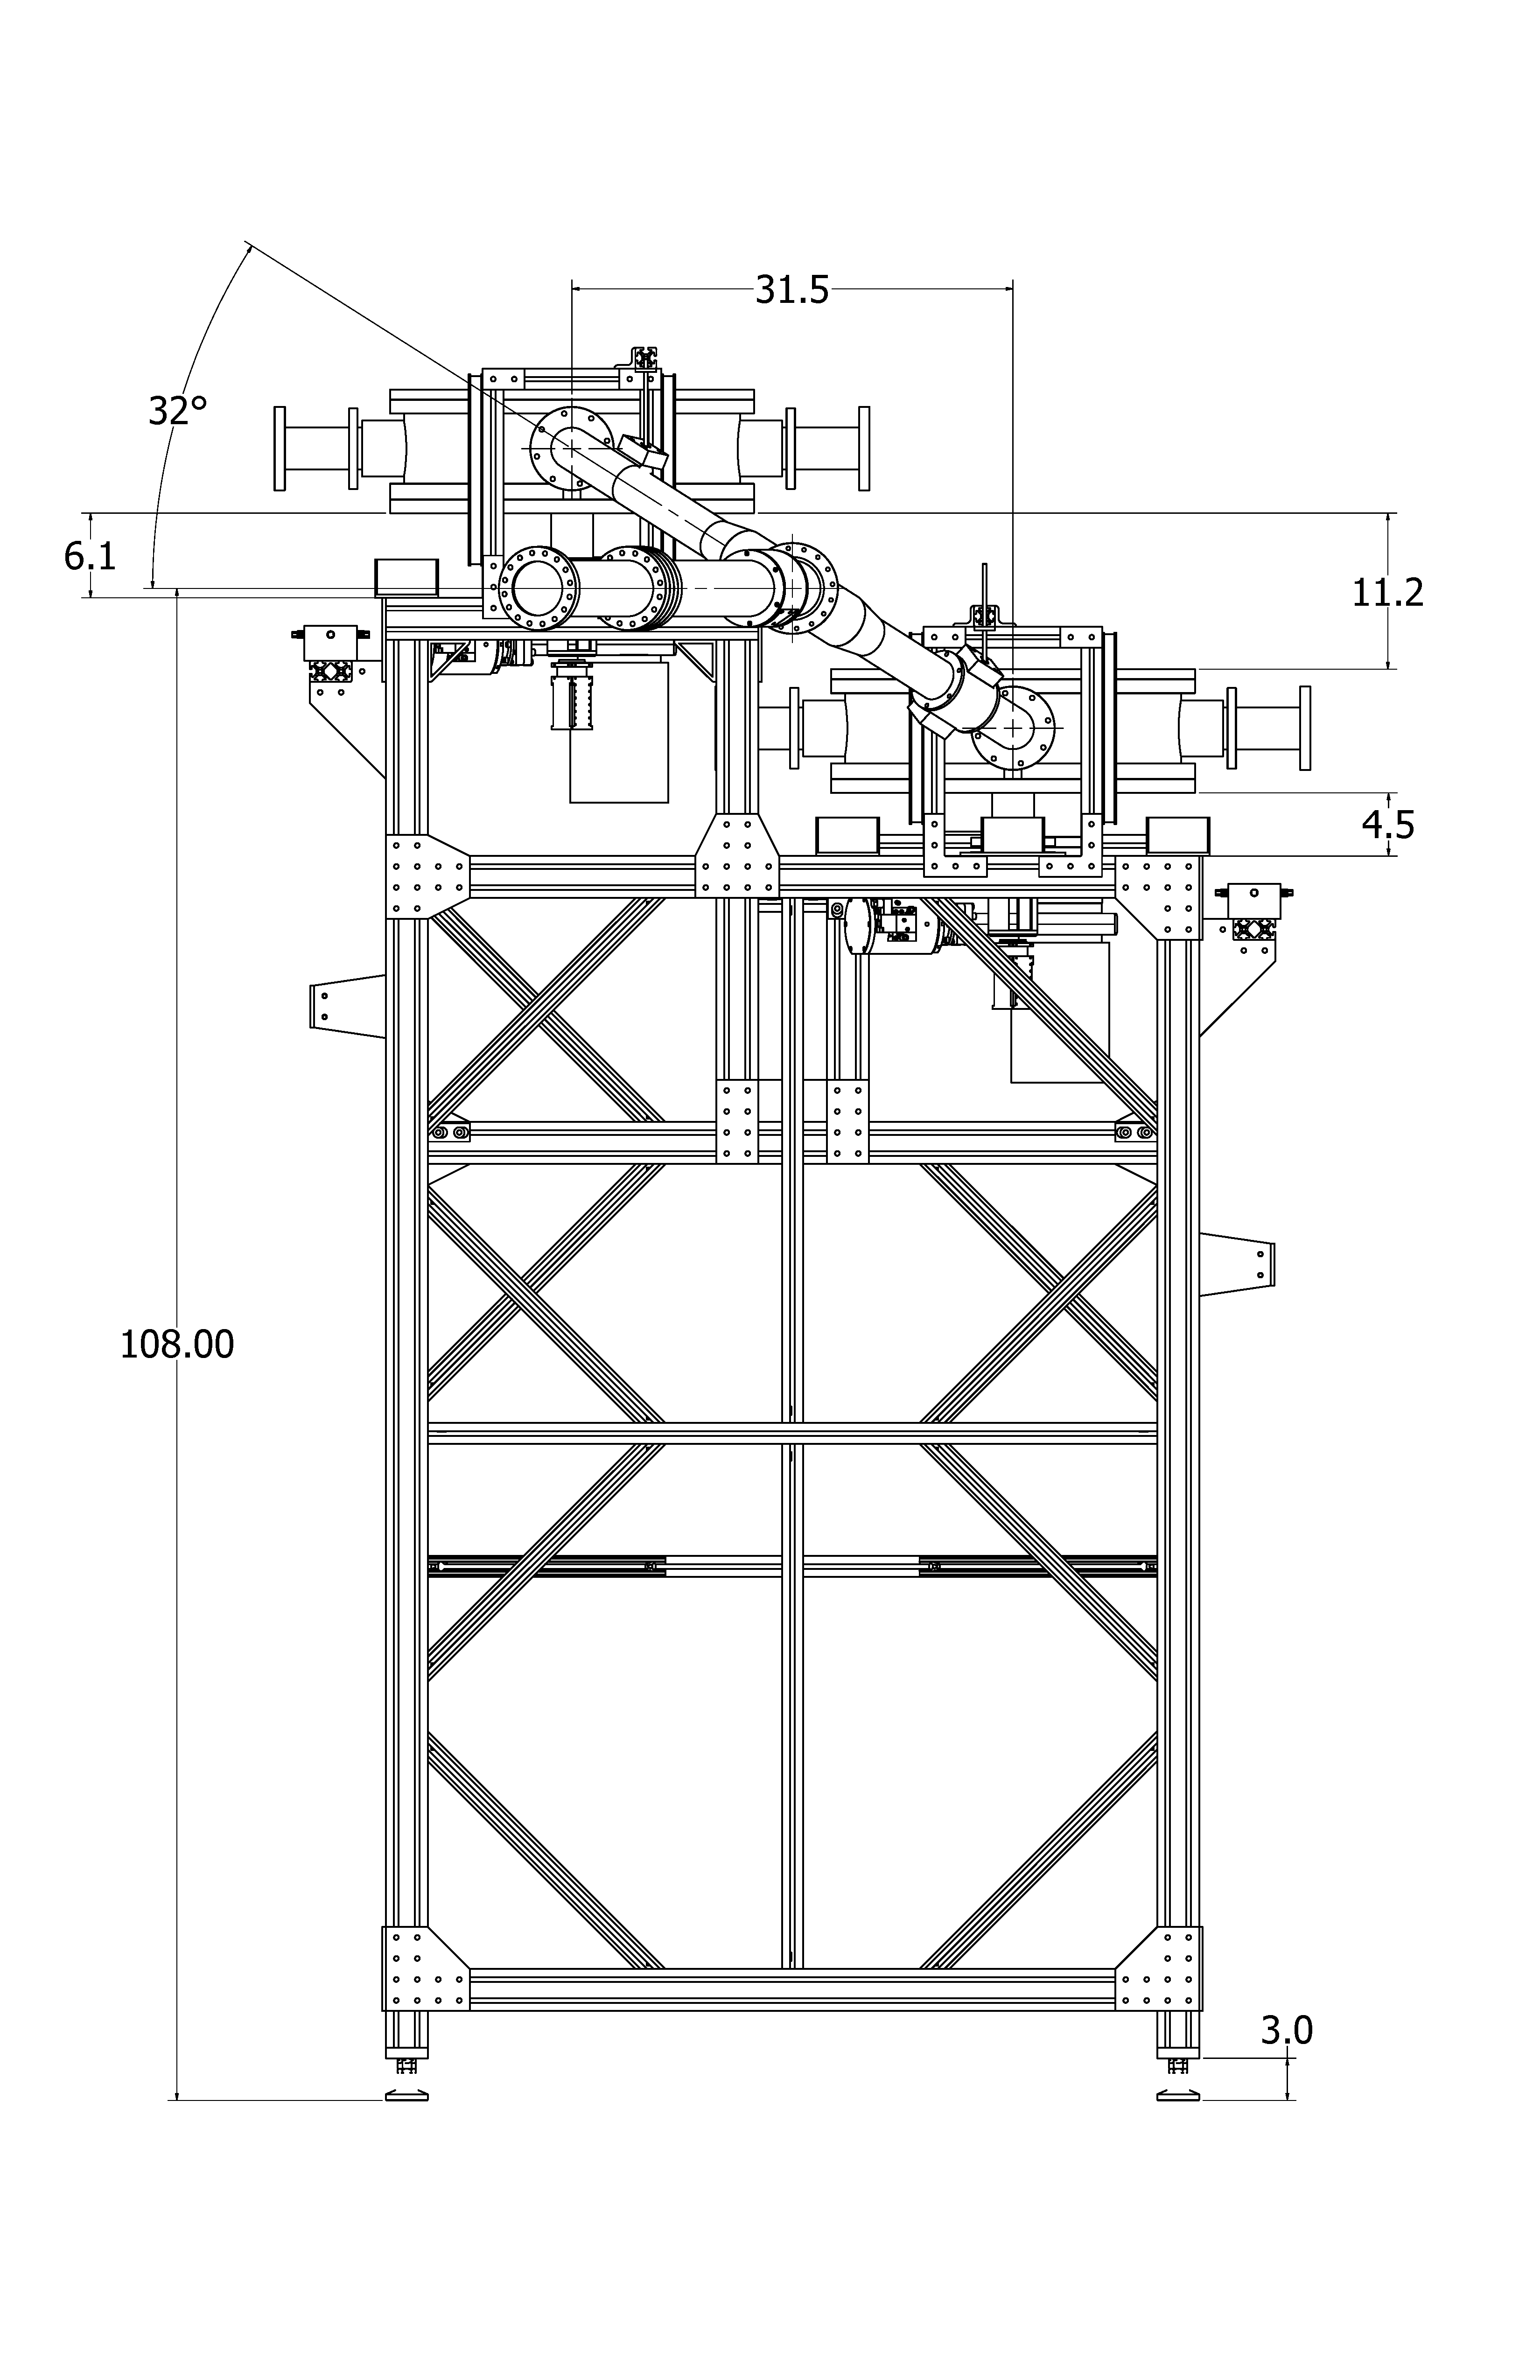
\includegraphics[width=3.5in]{figures/switcher_verticals.pdf}
    \caption
    {Schematics for switcher stand and switcher wye. Dimensions are in inches. Courtesy of Mark Luxnat.}
    \label{fig:switcher_stand_measurements}
\end{sidewaysfigure}


\begin{figure}
\centering
%subfigure width gets "multiplied" by includegraphics width
\begin{subfigure}{.5\textwidth}
  \centering
  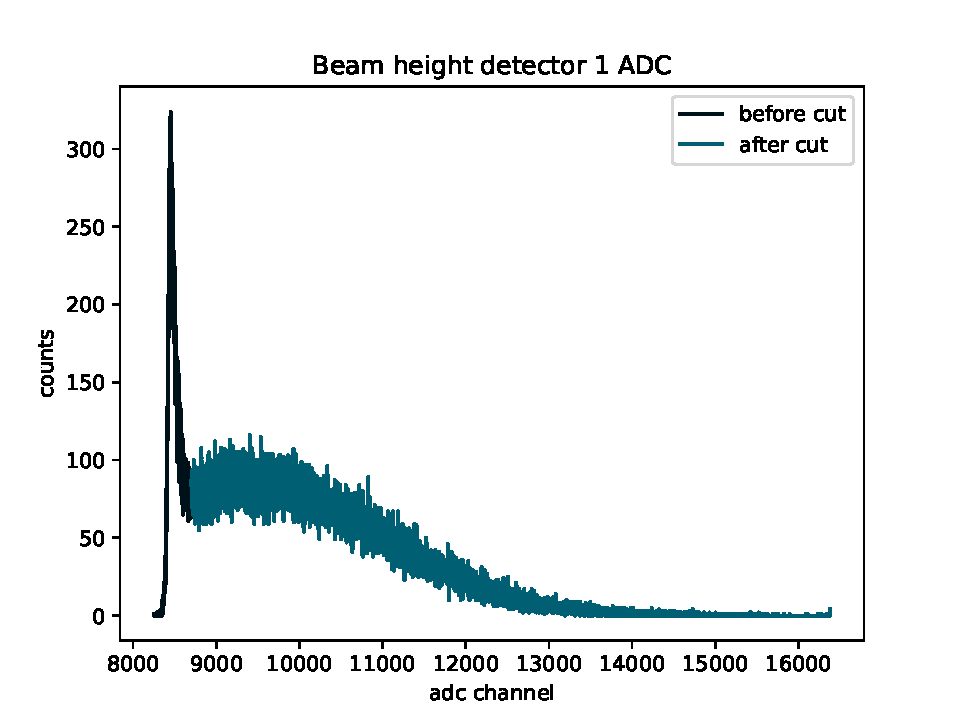
\includegraphics[width=\textwidth]{figures/2021_beam_det_1_adc.pdf}
  \caption{}\label{subfig:beam_det_1_adc}
\end{subfigure}%DO NOT REMOVE THIS '%'
\begin{subfigure}{.5\textwidth}
  \centering
  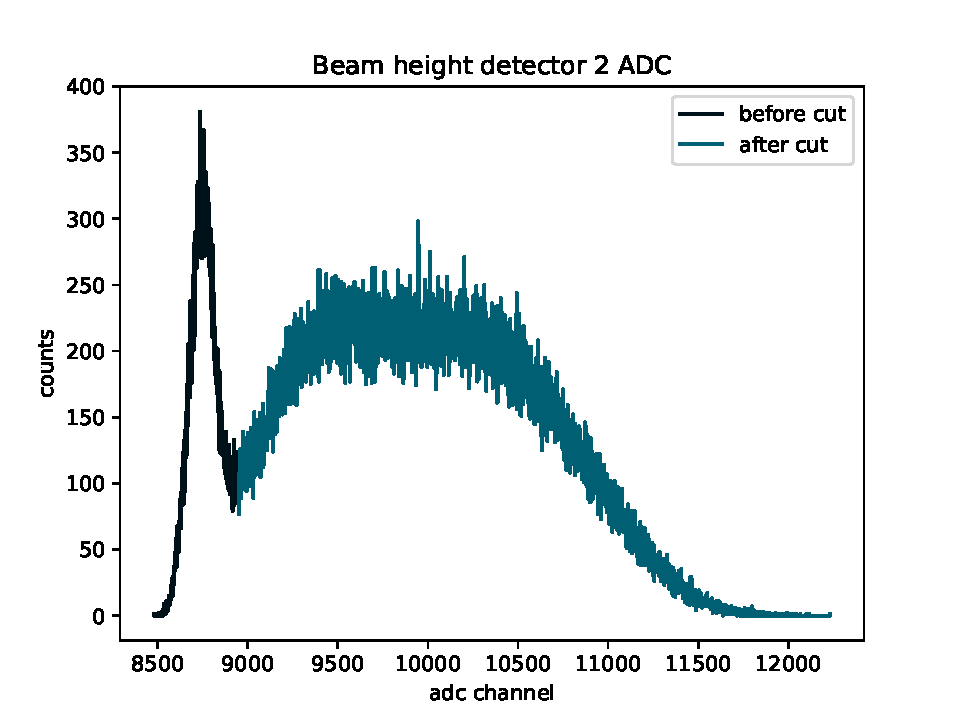
\includegraphics[width=\textwidth]{figures/2021_beam_det_2_adc.pdf}
  \caption{}\label{subfig:beam_det_2_adc}
\end{subfigure}
\begin{subfigure}{.5\textwidth}
  \centering
  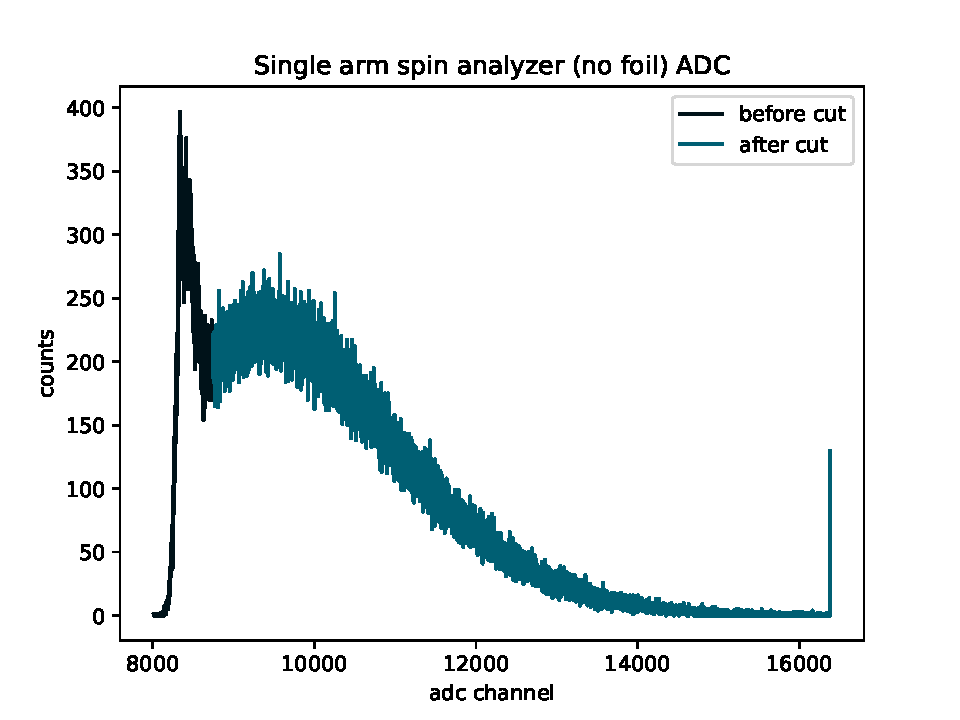
\includegraphics[width=\textwidth]{figures/2021_single_arm_no_foil_adc.pdf}
  \caption{}\label{subfig:single_arm_no_foil_adc}
\end{subfigure}
\caption
[Peak height spectra from \BZnS scintillator and PMT detectors (additional data acqusition details in Chap.~\ref{chap:daq}).]
{Peak height spectra from \BZnS scintillator and PMT detectors (additional data acqusition details in Chap.~\ref{chap:daq}). \textbf{(\subref{subfig:beam_det_1_adc})}--\textbf{(\subref{subfig:beam_det_2_adc})} Beam height detectors. \textbf{(\subref{subfig:single_arm_no_foil_adc})} Drop detector with polarizing foil removed. The largest bin in the histogram $x$-axis ($2^{14}-1$) includes counts of pulse heights greater than the range of the histogram}
\label{fig:2021_detector_adc}
\end{figure}

%%%%%%%%%%%%%%%%%%%%%%%%%%%%%%%%%%%%%%%%%%%%%%

\section{UCN transport measurements}\label{sec:2021_ucn_transport_switchers}

%%%%%%%%%%%%%%%%%%%%%%%%%%%%%%%%%%%%%%%%%%%%%%

For the first \ucn transport measurement, two beam height detectors were mounted on the upper switcher. The West GV was opened and the roundhouse was filled with \ucn for \qty{300}{s}, after which the roundhouse GV was opened. \ucn were flowed into the first beam height detector for \qty{80}{s}, to allow the \ucn gas in the guide to reach pseudo-equilibrium, before being counted for \qty{20}{s}. The upper switcher was then rotated to direct \ucn from the wye to the second beam height detector. A second \qty{20}{s} counting period was then performed. For the entire duration of the measurement the lower switcher directed \ucn from the wye into the single channel spin analyzer. To allow for comparison with the beam height detectors, the polarizing foil in the drop detector was removed (\BZnS scintillator diameter of \qty{3}{in}).

For the second \ucn transport measurement, one beam height detector was mounted on the upper switcher, and one was mounted on the lower switcher. The lower switcher directed \ucn from the wye to the drop detector. As with the first measurement, the roundhouse was filled for \qty{300}{s}, and the first \qty{20}{s} counting period was started \qty{80}{s} after the opening of the roundhouse GV. After the first counting period, the lower switcher was rotated to direct \ucn from the wye to the attached beam height detector. This was followed by a second \qty{20}{s} counting period.

The peak height spectra for the beam height detectors and the drop detector with foil removed is shown in Fig.~\ref{fig:2021_detector_adc}. For detected \ucn incident on a thick \BZnS scintillator the peak high spectra has an identifiable noise peak~\cite{jeph_multilayer_2015}, and we applied cuts to the data. The peak height spectra and corresponding data cuts did not change between measurement configurations. Counted \ucn were normalized using the West GV monitor rate similar to Chaps.~\ref{chap:north_beamline_paper}--\ref{chap:ssa_2020}. 

The result of the transport measurements is depicted in Tab.~\ref{tb:2021_transport}. When both beam height detectors were on the upper switcher, they exhibited comparable count rates. When beam height detector 1 was moved from the upper switcher to the lower switcher, it observed a factor of $\approx 1.5$ increase in the UCN rate. 

Such a discrepancy in transmission appeared to be too large to attribute solely to the geometry of the wye. For a $v^2\,dv\,(=E^{1/2}\,dE)$ or $v^3\,dv\,(=E\,dE)$ input distribution of UCN (Sec.~\ref{subsec:storageCurves}) and a maximum containing optical potential of \qty{188}{\nano\eV} (due to exposed stainless steel, as discovered in Sec.~\ref{sec:single_arm_flow_through_west_2021}), the fraction of UCN rejected by the \qty{25}{\eV} gravitational potential step from the elevation of the upper switcher is
%
\begin{gather}
    \frac{\int_{\qty{0}{neV}}^{\qty{190}{neV}}E^{1/2}\,dE}{\int_{\qty{25}{neV}}^{\qty{190}{neV}}E^{1/2}\,dE} < 1.5 \label{eq:switcher_transmission_issue}
\end{gather}
%
For Eq.~(\ref{eq:switcher_transmission_issue}) to approach 1.5, the containing optical potential had to be similar to Al (\qty{54}{\nano\eV} in Tab.~\ref{tb:optical_potentials}), which led to the suspicion that there was exposed Al in the wye. However, as demonstrated by Monte Carlo simulations, the assumptions made about UCN energy distribution per detector simply do not hold, and the the geometry of the switcher wye and roundhouse alone was found to be sufficient to reproduce the discrepancy. The simulation and results are described in Sec.~\ref{sec:switcher_height_monte_carlo}.

% \begin{table}
%     \centering
%     \caption{West beamline UCN transport measurement through the switcher wye and switchers}\label{tb:2021_transport}
%     \begin{tabular}{
%         l  
%         p{2in}
%         p{2in}
%     }
%     \toprule
%         & {\small Beam height 1 on upper switcher, Beam height 2 on upper switcher} & {\small Beam height 1 on lower switcher, Beam height 2 on upper switcher} \\
%     \midrule
%         & {Normalized count rate} & {Normalized count rate} \\
%         & {[\unit{UCN\per \second}]} & {[\unit{UCN\per \second}]} \\
%     \midrule
%         Beam height 1 &  1483(7) & 2283(9)\\
%         Beam height 2 &  1479(9) & 1513(6)\\
%         Drop detector (no foil) & 1532(5) & 1450(10)\\
%     \bottomrule
%     \end{tabular}
% \end{table}

\begin{table}
    \centering
    \caption{West beamline UCN transport measurement through the switcher wye and switchers. Detector counts were normalized to the average West GV monitor rate}\label{tb:2021_transport}
    \begin{tabular}{
        p{2in} 
        c
        c
        c
    }
    \toprule
        {Run condition} & {Beam height 1} & {Beam height 2} &{Drop det. (no foil)} \\
        & {$[\unit{UCN\per s}]$} & {$[\unit{UCN\per s}]$} & {$[\unit{UCN\per s}]$}\\
    \midrule
        {\small Beam height 1 on upper switcher Beam height 2 on upper switcher} &  1483(7) & 1479(9) & 1532(5)\\
        \\
        {\small Beam height 1 on lower switcher Beam height 2 on upper switcher} &  2283(9) & 1513(6) & 1450(10)\\
    \bottomrule
    \end{tabular}
\end{table}

%%%%%%%%%%%%%%%%%%%%%%%%%%%%%%%%%%%%%%%%%%%%%%

\section{Spin asymmetry measurements}\label{sec:asymmetry_west_2021}

%%%%%%%%%%%%%%%%%%%%%%%%%%%%%%%%%%%%%%%%%%%%%%

%%%%%%%%%%%%%%%%%%%%%%%%%%%%%%%%%%%%%%%%%%%%%%

\subsection{Flow-through spin asymmetry measurement}\label{sec:single_arm_flow_through_west_2021}

%%%%%%%%%%%%%%%%%%%%%%%%%%%%%%%%%%%%%%%%%%%%%%

The spin asymmetry flow-through measurement from Sec.~(\ref{sec:ssa_measurements}) was repeated for the drop detector on the lower switcher (polarizer reinstalled). The RF was incremented every \qty{30}{s} and the counting period was set in the middle \qty{20}{s} of each step.  The upper switcher directed \ucn from the wye to a beam height detector. The asymmetry calculated from Eq.~(\ref{eq:spin_asymmetry}) is given in Fig.~\ref{fig:2021_west_single_arm_asymmetry}, with the maximal asymmetry $A\approx 0.15$. By comparison, same drop detector on previous North beamline measurements (Fig.~\ref{fig:spin_flipper_efficiency}) had an asymmetry of $A\approx 0.8$.

Investigation with the assistance of UCN$\tau$ collaborators revealed the existence of exposed stainless steel components in the roundhouse from modifications prior to the measurements in this chapter. Relative to other UCN friendly surfaces, stainless steel is known to have a higher depolarization per bounce. 

A similar asymmetry measurement using the UCN$\tau$ magneto-gravitational trap as a spin-analyzer (production runs \#21184, \#21187) gave $A\approx 0.3$. It is of note that the UCN$\tau$ trap cannot store \ucn of energy $>\qty{100}{neV}$, whereas, assuming there is no issue with the coating, the NiP surfaces in the switcher wye and switchers should be capable of storing UCN up to $\qty{213}{neV}$. Higher energy UCN have shorter polarization lifetimes due to a larger number of bounces in the storage volume. Therefore, comparison of the drop detector asymmetry ($A\approx 0.15$) to the UCN$\tau$ asymmetry was found to be consistent with assumption that the roundhouse was the primary cause of depolarization, and not one of the commissioned nEDM beamline components.


%%%%%%%%%%%%%%%%%%%%%%%%%%%%%%%%%%%%%%%%%%%%%%%%%%%%%%%%%%%%

\subsection{Roundhouse fill and unload asymmetry measurement}

%%%%%%%%%%%%%%%%%%%%%%%%%%%%%%%%%%%%%%%%%%%%%%%%%%%%%%%%%%%

\begin{figure}
\centering
\begin{minipage}{.47\textwidth}
    \centering
    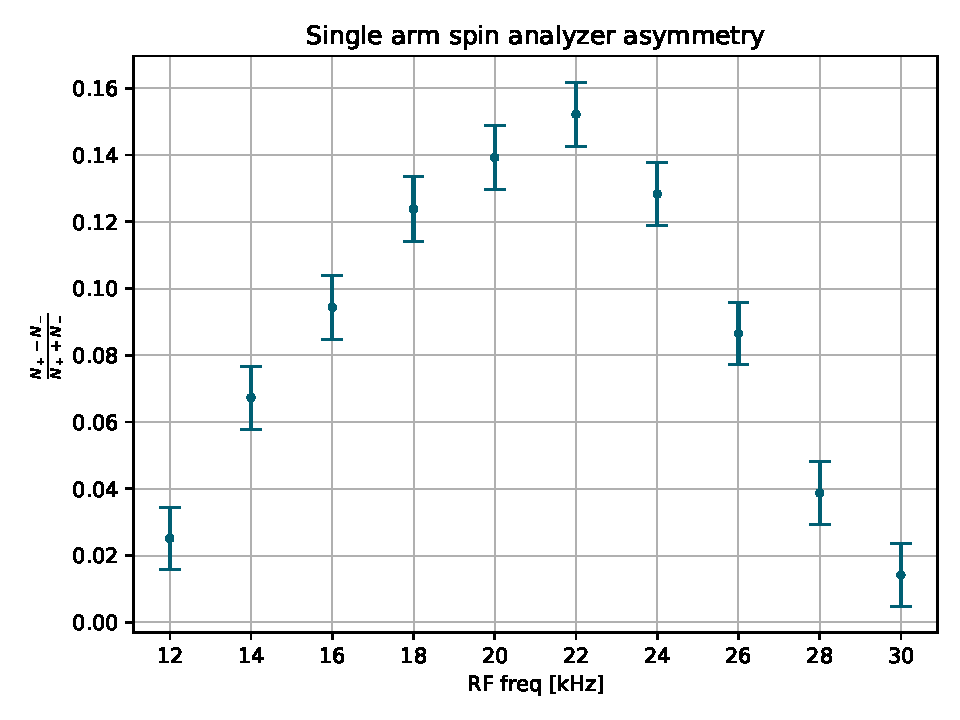
\includegraphics[width=\textwidth]{figures/single_arm_asymmetry_2021.pdf}
    \caption
    {Spin asymmetry measurement with the drop detector, with UCN in a flow through mode from the source through the roundhouse to the detector (Sec.~\ref{sec:single_arm_flow_through_west_2021}).}
    \label{fig:2021_west_single_arm_asymmetry}
\end{minipage}%
\hspace{7pt}
\begin{minipage}{.47\textwidth}
    \centering
    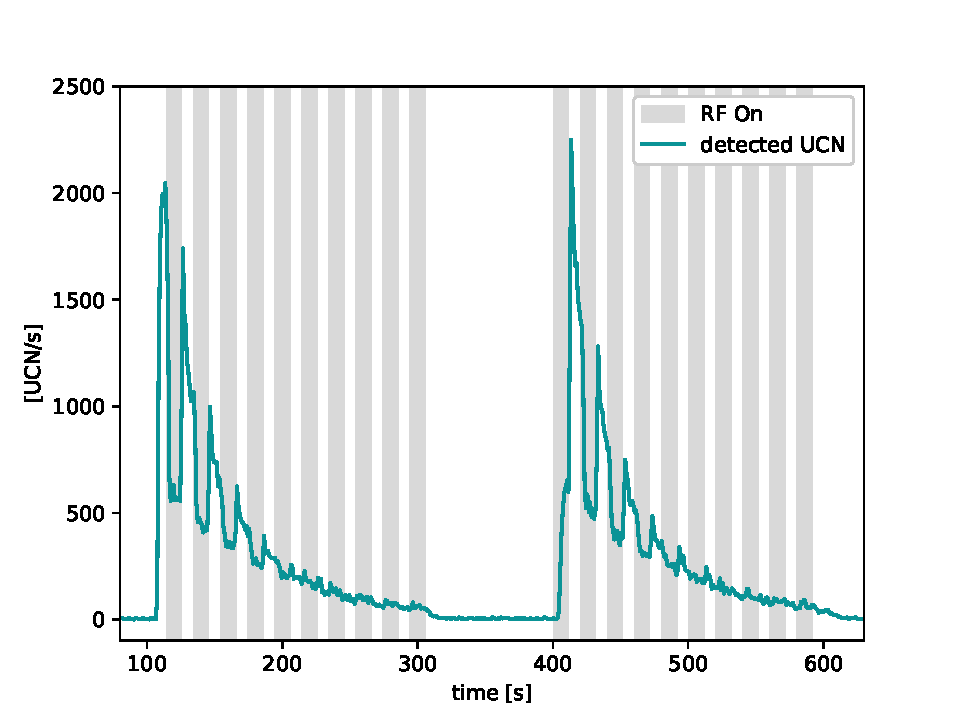
\includegraphics[width=\textwidth]{figures/2021_roundhouse_rf_toggle.pdf}
    \caption
    {Neutron count rate from a fill-and-dump run doublet from the roundhouse on the West beamline with the RF spin flipper toggling.}
    \label{fig:roundhouse_rf_toggle_doublet}
\end{minipage}
\end{figure}


In order to characterize spin transport through the switcher wye and lower (new) switcher, a method similar to the T1 asymmetry measurement in Chap.~\ref{chap:lanl_ramsey_demonstration} was adopted. The motivation behind this series of measurements was twofold. First, it would be meaningful for the LANL UCN program to gain information regarding the depolarizing nature of the roundhouse. Second, the remaining accelerator production schedule 2021 did not allow for the time-consuming removal process of the stainless steel roundhouse components.

The roundhouse was filled for some variable period with the roundhouse GV closed, after which the UCN were dumped into the drop detector via switcher wye with the RF spin flipper toggling in \qty{10}{s} intervals. This counting period continued until the roundhouse was emptied ($\sim\qty{200}{s})$. Each fill-and-dump run was performed as a run doublet (Fig.~\ref{fig:roundhouse_rf_toggle_doublet}), where a run would begin with spin flipper off (on) before periodic toggling. Asymmetry was then calculated by comparing integrated counts per toggle in the run doublet, with counts normalized to the West GV monitor. 
 
Fig.~\ref{fig:2021_roundhouse_asymmetry_1} summarizes the results of the measurement. We observed that as the roundhouse filling time increased, asymmetry decreased, consistent with expectations of the roundhouse being depolarizing. Multiple roundhouse holding field configurations were tested, including one mode where the solenoid was turned off, leaving only Earth's magnetic field. Predictably, the nominal configuration had the highest asymmetry compared to the other modes

In the nominal roundhouse holding field configuration, utilizing only the first 4 integration periods of the run doublet to resulted in a higher calculated asymmetry. This led to Fig.~\ref{fig:2021_roundhouse_asymmetry_2}, which plots the asymmetry as a function of unload time (i.e., how many integration periods were used to calculate asymmetry). As unload time increased, asymmetry predictably decreased. Longer unloading periods would allow UCN with more passes through the depolarizing roundhouse region to travel to the drop detector and be counted.

The result of the measurements in this section suggested that the roundhouse depolarization dominated over possible depolarization in the switcher wye or new switcher, and that these components would be acceptable for the 2022 engineering run on the North beamline.

 \begin{figure}
    \centering
    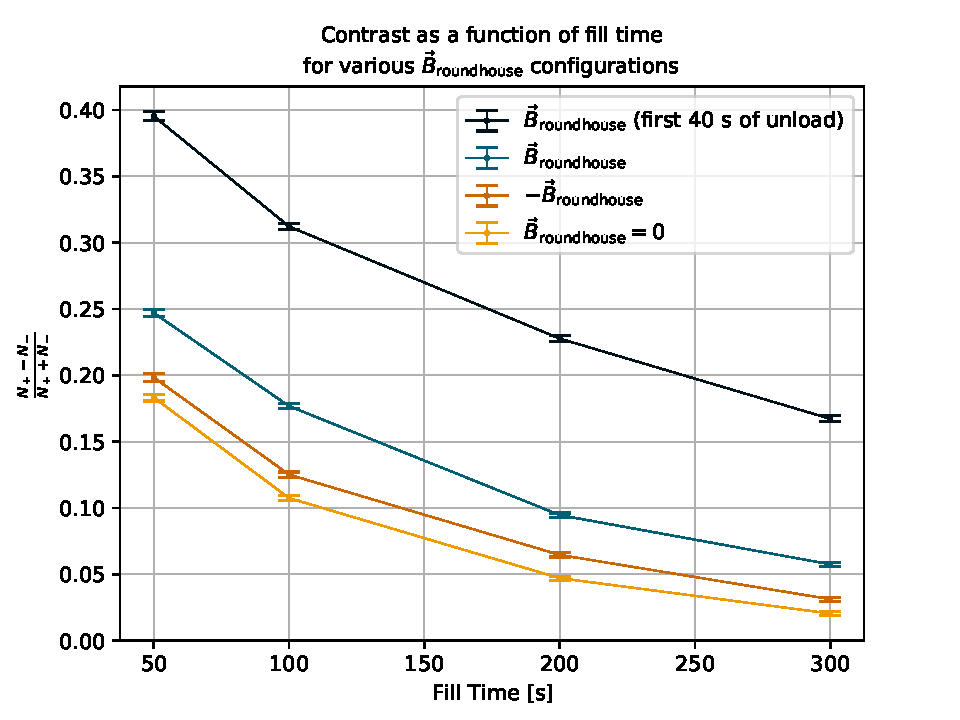
\includegraphics[width=0.6\textwidth]{figures/2021_roundhouse_asymmetry_1.pdf}
    \caption
    [Spin asymmetry from a fill-and-dump sequence of the roundhouse, where fill time was swept. The measurement was repeated for various orientations of the roundhouse magnetic holding field.]
    {Spin asymmetry from a fill-and-dump sequence of the roundhouse, where fill time was swept. The measurement was repeated for various configurations of the roundhouse magnetic holding field: nominal ($\vv{B}_\text{roundhouse}$), inverted along $z$ ($-\vv{B}_\text{roundhouse}$), and off ($\vv{B}_\text{roundhouse}=0$). The \legendbox{black} points labeled ``first 40 s of unload'' use the same data as the nominal configuration \legendbox{dark-blue-color}, but consider only the first 4 integration periods of the run doublet.}
    \label{fig:2021_roundhouse_asymmetry_1}
% \end{figure}
    \vspace{\baselineskip}
% \begin{figure}
    \centering
    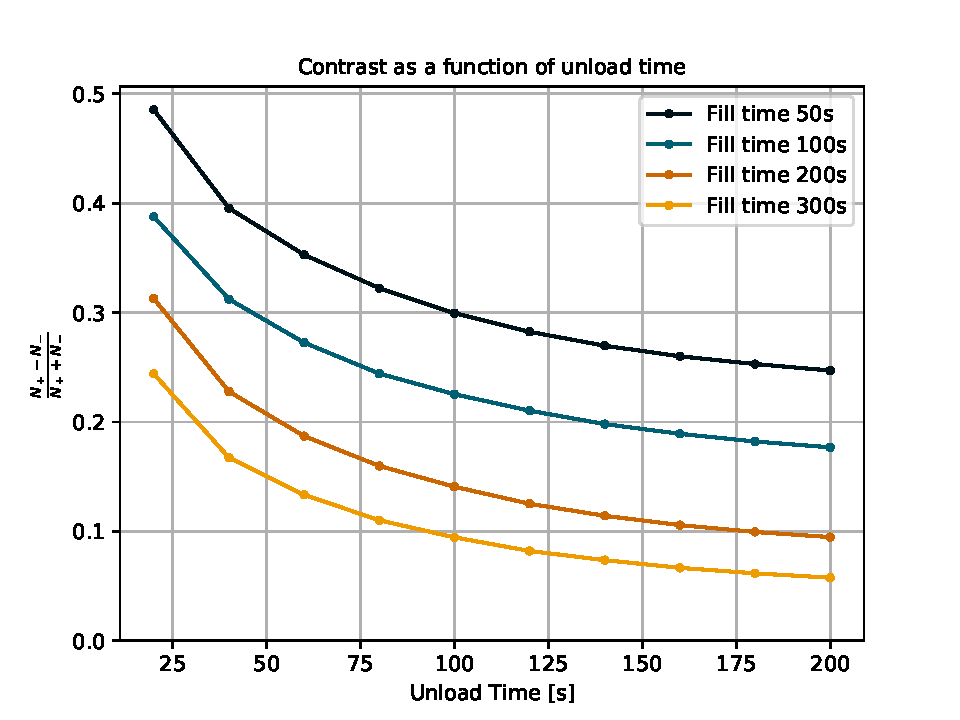
\includegraphics[width=0.6\textwidth]{figures/2021_roundhouse_asymmetry_2.pdf}
    \caption[Change in the asymmetry as the roundhouse unload progresses. The $x$-axis refers to the number of integration periods of the run doublet used to calculate asymmetry]
    {Change in the asymmetry as the roundhouse unload progresses. The $x$-axis refers to the number of integration periods of the run doublet used to calculate asymmetry (e.g., $\qty{20}{s}=$ first two integration periods,  $\qty{30}{s}=$ first three integration periods...).}\label{fig:2021_roundhouse_asymmetry_2}
\end{figure}